% Chapter Template

\chapter{Results} % Main chapter title

\label{Chapter3} % Change X to a consecutive number; for referencing this chapter elsewhere, use \ref{ChapterX}

%----------------------------------------------------------------------------------------
%	SECTION 1
%----------------------------------------------------------------------------------------
\section{Setup}

In this paper, we described a pipeline implemented using \texttt{python} then \texttt{C\#} and Unity’s real time development platform; as the visualization engine. To simulate fire behavior, we ran a Level set 4 FDS simulation, set to output plot3D files every 0.5 seconds on a 20m x 20m x 20m mesh, containing voxels 0.2m x 0.2m x 0.2m in size, with open boundary conditions. The simulation was 100 seconds in length with a ground fire igniting ten seconds into the simulation, a wind of 5.6 m/s originating from the south west (215\textdegree) and trees evenly distributed on the mesh. Figure \ref{fig:CFDTopDownSmokeview} shows a top down view of our visualization rendered in SmokeView, while Figure \ref{fig:CFDTopDownUnity} is the same visualization rendered in unity. \par 

The sample FDS input file and code used in this paper can be accessed at  \url{https://github.com/tjschweitzer/ReynoldsNumberSampling}.

\begin{figure}
\centering
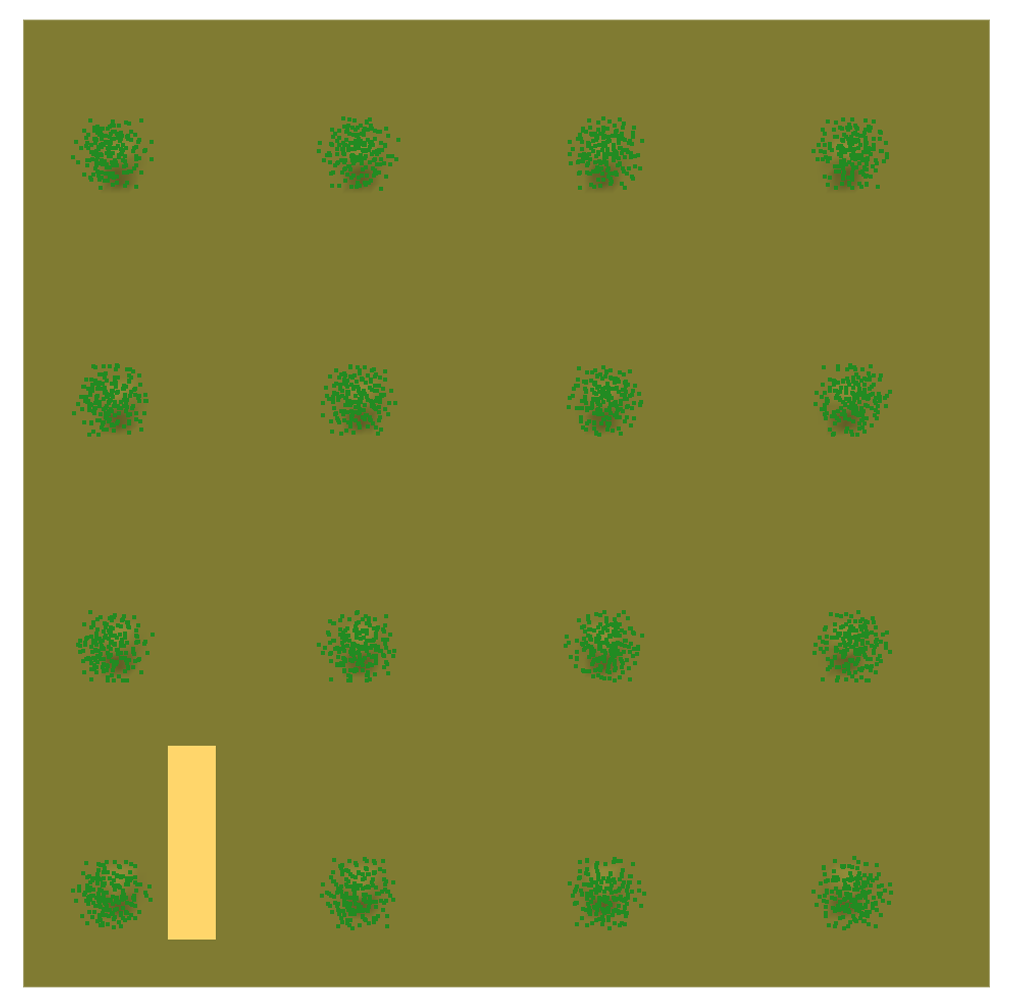
\includegraphics[scale=.3]{Figures/TopDownSMV.png}
\decoRule
\caption[Top Down SmokeView View]{A top-down view of the simulation in SmokeView }
\label{fig:CFDTopDownSmokeview}
\end{figure}
\begin{figure}
\centering
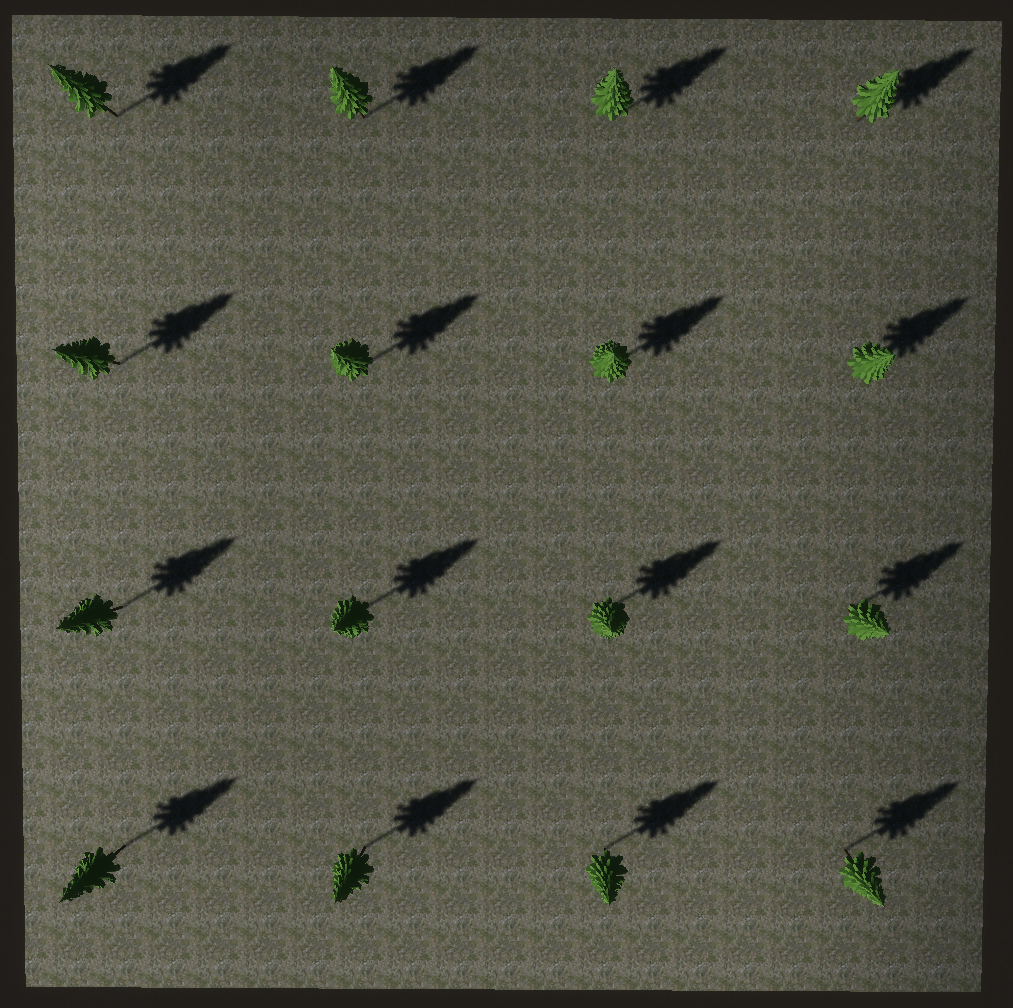
\includegraphics[scale=.3]{Figures/Topdown Unity.png}
\decoRule
\caption[Top Down Unity]{A top-down view of the simulation in Unity}
\label{fig:CFDTopDownUnity}
\end{figure}

\section{Analyses}

The CFD simulation was run using FDS 7.6.0, the total run time for this simulation took 252 (4 Hours 12 Min ) minutes to complete running 4 cores of an i7 4790k in parallel. The calculations discussed in this paper were able to complete in three minutes, with no parallelization.
Additionally, the size of the CFD output files was 5.0 Gigabytes, while the saved data needed for full virtual reality using our methodology is 28.9 Megabytes, a 99.4\% reduction in file size. When visualized inside of unity using a HMD ( HTC Vive and HTC Vive Pro was used during testing) we were able to average 15-30 frames per second with a resolution of 1440 x 1660 pixels per eye \ref{fig:LeftEye}, with the lowest frame rate during the transition between timesteps. This was achieved using an Intel i7 4790k CPU with a RTX 2070-Super GPU.


\begin{figure}
\centering
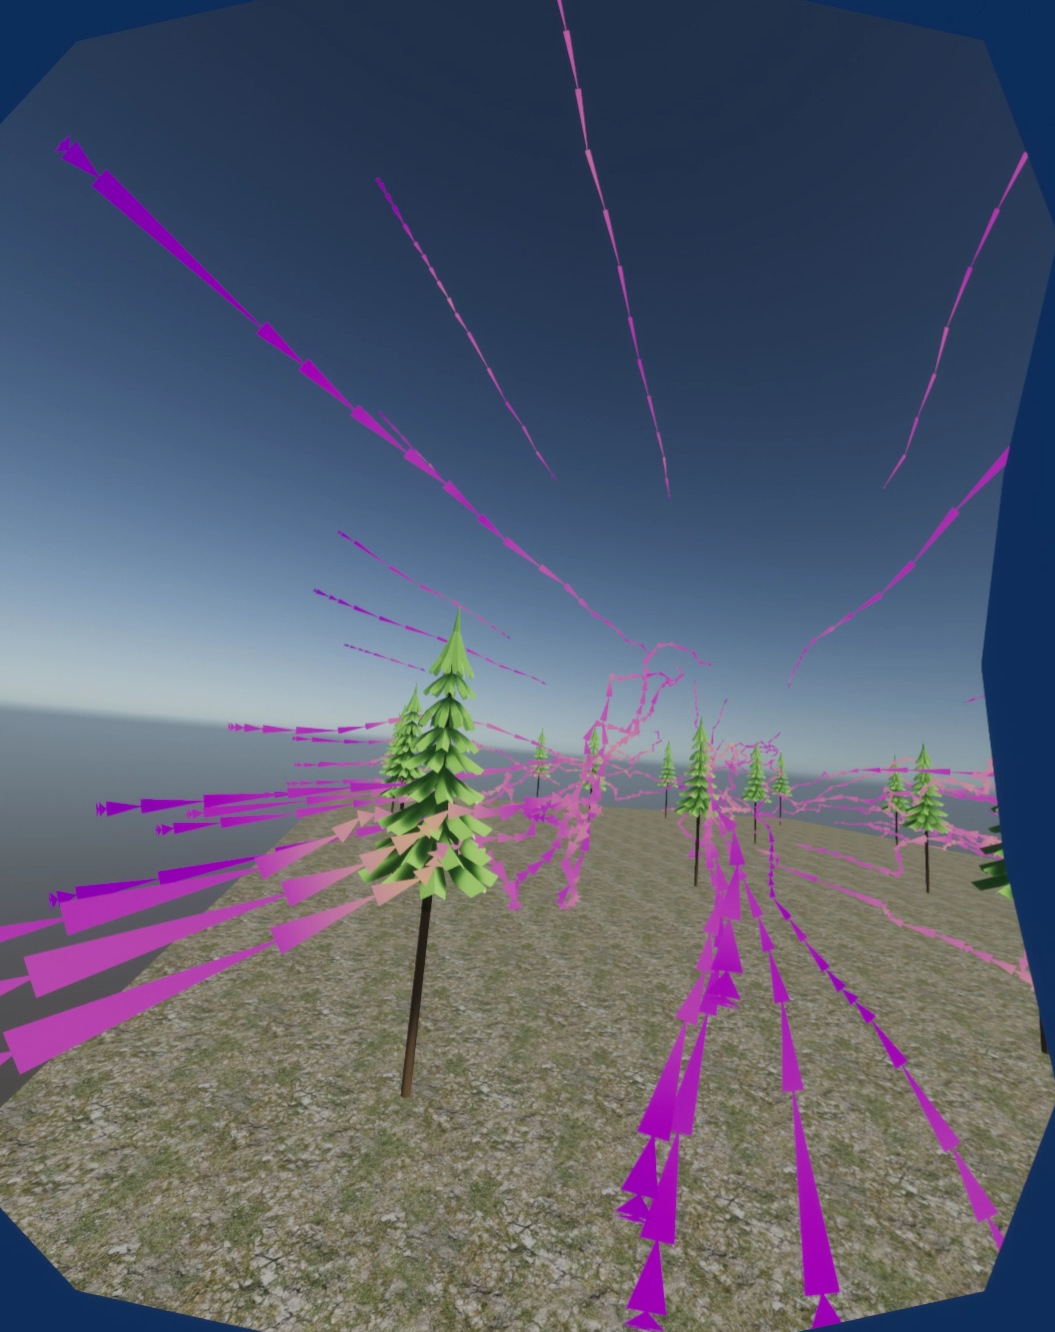
\includegraphics[scale=.29]{Figures/lefteye.png}
\decoRule
\caption[Unity View of Simulation]{A view of the video output to the left eye of a HMD from Unity}
\label{fig:LeftEye}
\end{figure}
\begin{figure}
\centering
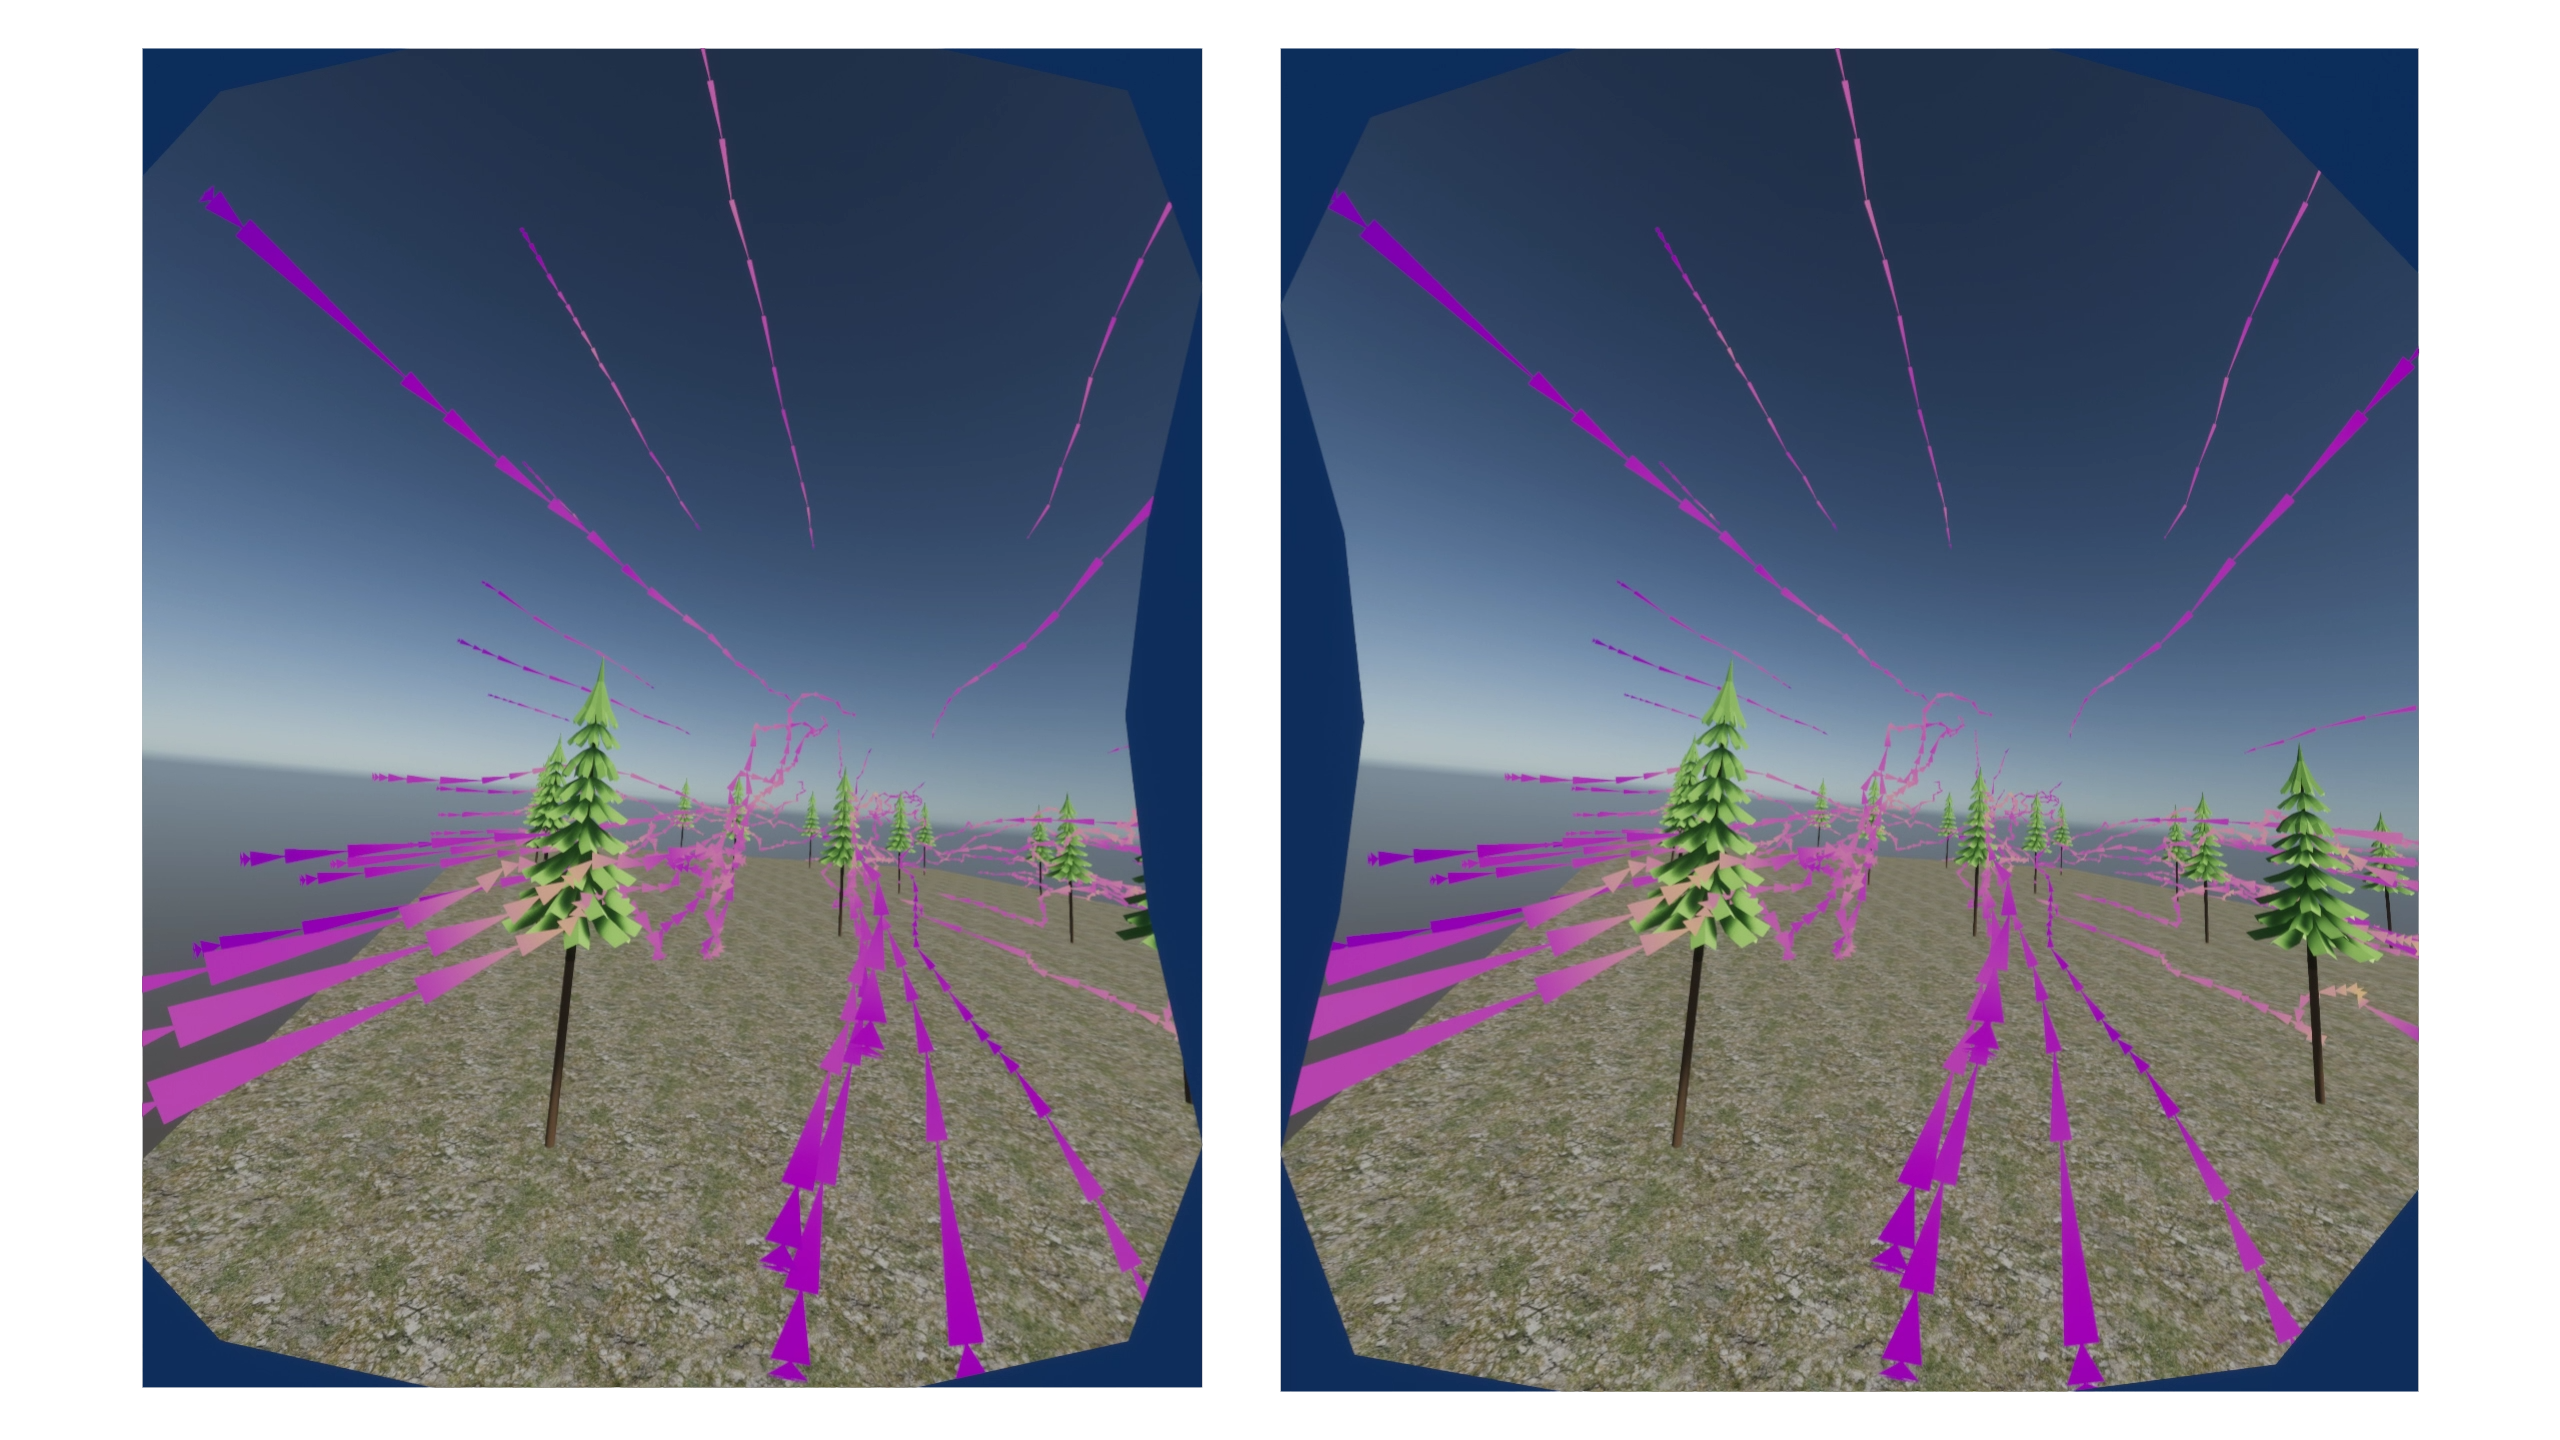
\includegraphics[scale=.18]{Figures/botheyes.png}
\decoRule
\caption[Unity View of Simulation]{A view of the video output to the eyes of a HMD from Unity}
\label{fig:AllEyes}
\end{figure}